\appendix

% ==============================================================================
% APÊNDICE A - PROMPTS
% ==============================================================================
\section{Prompts Utilizados no Experimento}
\label{apendice:prompts}

Para garantir a reprodutibilidade e transparência deste estudo, apresentamos a seguir a transcrição integral dos \textit{prompts} utilizados.

\subsection{Prompt para Geração de Dados Sintéticos (Golden Set)}
Este prompt foi utilizado para instruir o modelo GPT-4o a atuar como um analista de dados e gerar as 100 perguntas de teste.

\begin{promptbox}{System Instruction: Gerador de Dados Sintéticos}
  \small
  \textbf{\# CONTEXTO E PERSONA}\\
  Você é um analista de dados e especialista em legislação, encarregado de criar um rigoroso conjunto de avaliação para um sistema de chatbot de Inteligência Artificial (RAG). Sua tarefa é analisar os documentos legais do Ministério Público do Espírito Santo (MP-ES) fornecidos abaixo e gerar um conjunto diversificado e desafiador de pares de pergunta e resposta.

  \vspace{0.2cm} \hrule \vspace{0.2cm}

  \textbf{\# SIMULAÇÃO DE COMPORTAMENTO DO USUÁRIO}\\
  Formule as perguntas do ponto de vista de um usuário real que \textbf{NÃO SABE} em qual documento ou link a resposta se encontra.
  \begin{itemize}
    \item As perguntas devem ser naturais e gerais.
    \item \textbf{NUNCA} inclua o link da fonte ou qualquer nome de arquivo no texto da pergunta.
    \item A fonte (o link) deve ser usada APENAS para preencher o campo \texttt{"source"} no JSON de saída.
  \end{itemize}

  \vspace{0.2cm} \hrule \vspace{0.2cm}

  \textbf{\# TAREFA PRINCIPAL}\\
  Com base EXCLUSIVAMENTE no conteúdo dos documentos fornecidos, gere um total de \textbf{40 perguntas}, divididas igualmente entre as 4 categorias a seguir (10 perguntas por categoria):
  \begin{enumerate}
    \item \textbf{FATUAL:} "Qual o prazo para a interposição de recursos?".
    \item \textbf{SÍNTESE:} "Quais são as diferenças entre os procedimentos de férias e licença-prêmio?".
    \item \textbf{PROCEDIMENTAL:} "Descreva o procedimento para solicitar o teletrabalho.".
    \item \textbf{AGULHA NO PALHEIRO:} "Qual o valor exato do auxílio-alimentação citado?".
  \end{enumerate}

  \vspace{0.2cm} \hrule \vspace{0.2cm}

  \textbf{\# FORMATO DA SAÍDA}\\
  Sua resposta final deve ser APENAS um array JSON válido, sem introduções, seguindo o esquema abaixo.
\end{promptbox}

\begin{jsonbox}{Esquema JSON Esperado (Output)}
  [
    {
      "id": "ID_UNICO",
      "category": "NOME_DA_CATEGORIA",
      "question": "TEXTO DA PERGUNTA (GERAL)",
      "ground_truth_answer": "RESPOSTA COMPLETA E IDEAL",
      "evidence_quote": "CITACAO EXATA DO DOCUMENTO",
      "source": "http://link.da.fonte.gov.br/documento"
    }
  ]
\end{jsonbox}

\noindent \textit{Nota: O conteúdo dos documentos reais foi inserido dinamicamente no final do prompt durante a execução do script.}

\newpage

\subsection{System Prompt do Assistente RAG}
Este é o comando de instrução (\textit{system role}) passado ao modelo durante a fase de inferência.

\begin{promptbox}{System Role: Assistente Jurídico MPES}
  \small
  "Você é um Assistente Jurídico Virtual do Ministério Público do Estado do Espírito Santo. Sua função é auxiliar servidores e cidadãos a entenderem os atos normativos da instituição.

  \textbf{Diretrizes de Resposta:}
  \begin{itemize}
    \item Baseie sua resposta \textbf{EXCLUSIVAMENTE} no contexto fornecido (trechos recuperados). Não use seu conhecimento prévio para inventar leis.
    \item Sempre cite a fonte normativa (ex: 'Conforme o Art. 5º da Portaria Nº 123...').
    \item Se o contexto não contiver a informação necessária, diga: \textit{'Desculpe, o contexto recuperado não contém informações suficientes sobre este tema.'} Não tente adivinhar.
    \item Mantenha um tom formal, objetivo e impessoal."
  \end{itemize}
\end{promptbox}

% ==============================================================================
% APÊNDICE B - INTERFACE DO PORTAL MPES
% ==============================================================================
\newpage
\section{Interface do Portal de Legislação do MPES}
\label{apendice:portal}

A Figura \ref{fig:portal_mpes} apresenta a interface de busca e os diversos filtros (como espécie normativa, tema, situação e autor) do portal oficial de legislação do MPES. Esta interface foi utilizada como fonte primária para o processo de \textit{web scraping} e composição do \textit{corpus} documental deste trabalho.

\begin{figure}[htbp]
  \centering
  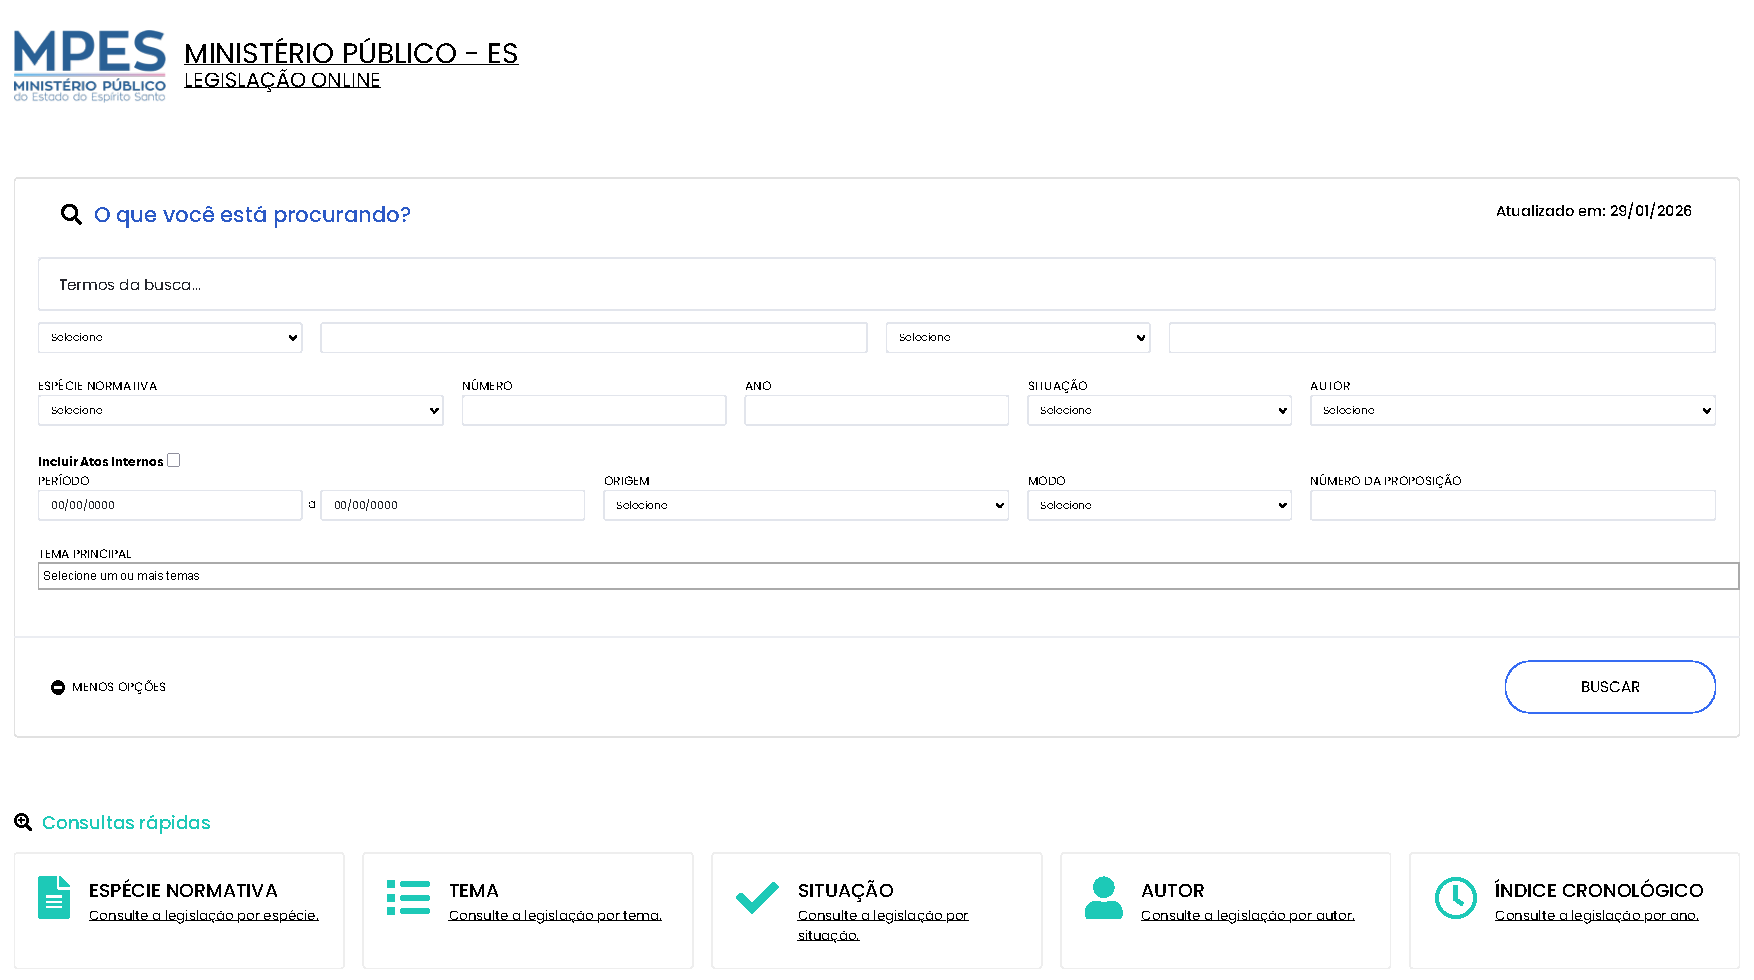
\includegraphics[width=1\linewidth]{figuras/portal_cropped.pdf}
  \caption{Captura de tela do Portal de Legislação Online do MPES.}
  \label{fig:portal_mpes}
\end{figure}

% ==============================================================================
% APÊNDICE C - INTERFACE DA ASSISTENTE FABI
% ==============================================================================
\newpage
\section{Interface da Assistente Virtual Fabi}
\label{apendice:interface_fabi}

A Figura \ref{fig:print_fabi} ilustra o ambiente de testes da assistente virtual Fabi. A interface permite que o usuário realize perguntas em linguagem natural e receba respostas sintetizadas que incluem a citação direta das fontes normativas consultadas, garantindo a rastreabilidade da informação.

\begin{figure}[htbp]
  \centering
  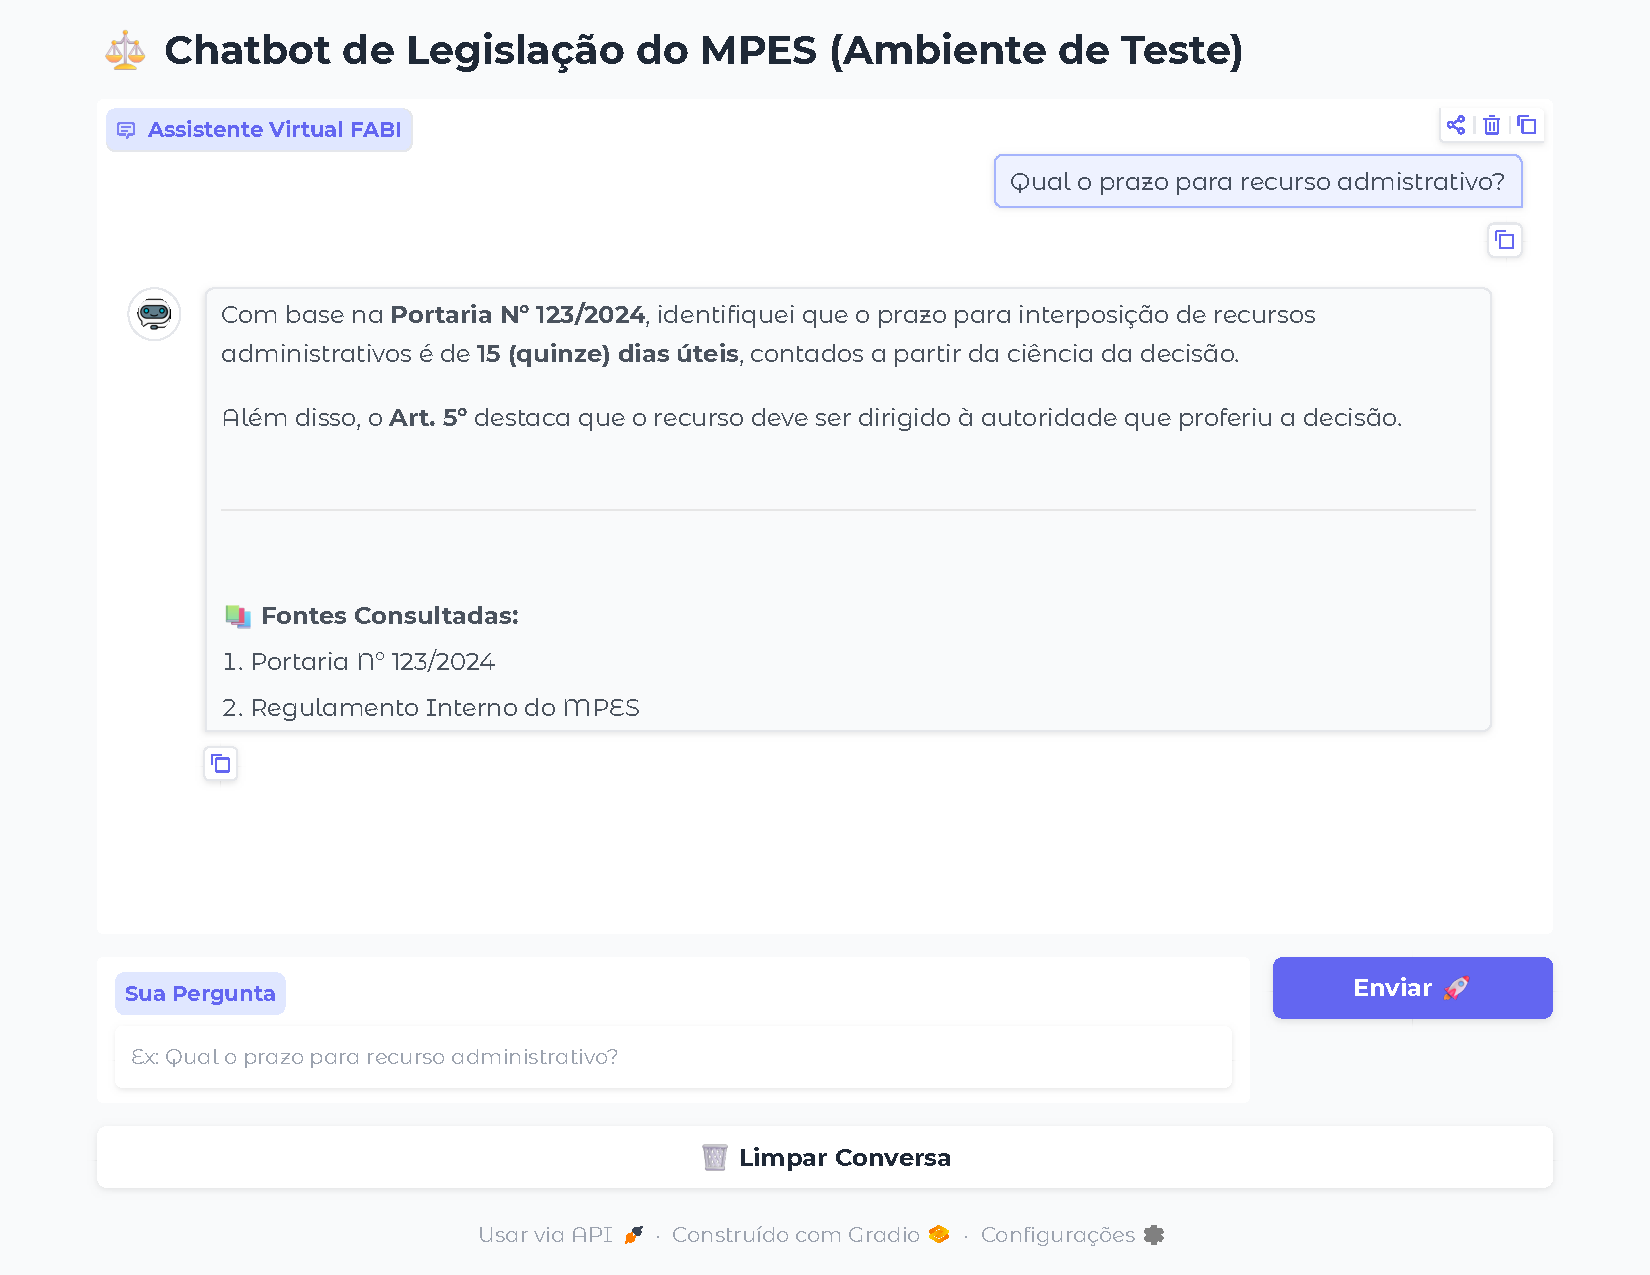
\includegraphics[width=0.6\linewidth]{figuras/Fabi.pdf}
  \caption{Interface de interação da assistente Fabi desenvolvida com o framework Gradio.}
  \label{fig:print_fabi}
\end{figure}

% ==============================================================================
% APÊNDICE D - INTERFACE DA API (SWAGGER UI)
% ==============================================================================
\newpage
\section{Interface de Documentação da API (Swagger UI)}
\label{apendice:api}

A Figura \ref{fig:print_api} apresenta a interface de documentação interativa (Swagger UI) gerada automaticamente pelo \textit{framework} FastAPI para o orquestrador do sistema RAG. A imagem detalha o \textit{endpoint} de requisição principal (\texttt{POST /responder}) e o esquema de dados JSON (\textit{payload}) utilizado para parametrizar as inferências, permitindo o controle rigoroso de hiperparâmetros experimentais como \texttt{top\_k}, \texttt{chunking\_strategy}, \texttt{search\_type} e o modelo gerador (\texttt{model}).

\begin{figure}[htbp]
  \centering
  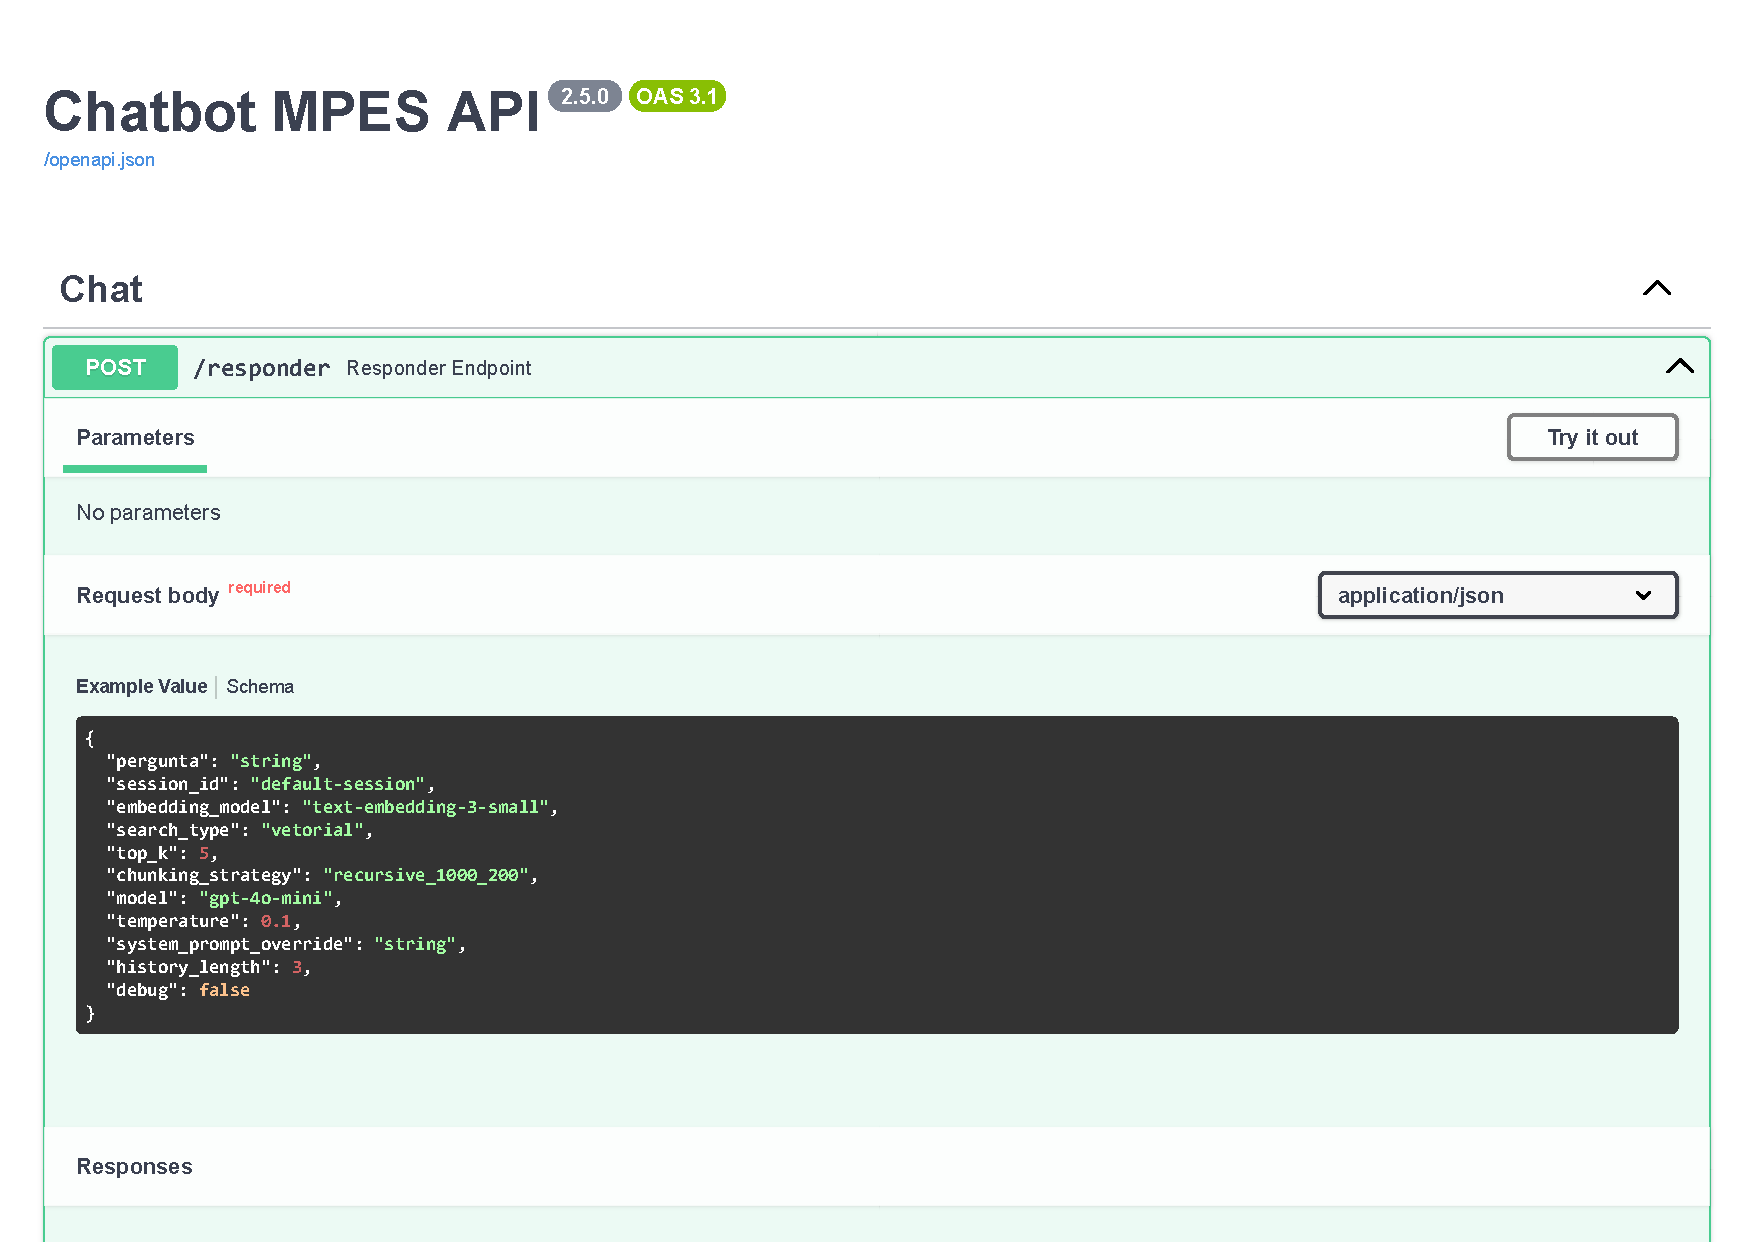
\includegraphics[width=0.9\linewidth]{figuras/api.pdf}
  \caption{Interface de documentação da API do Chatbot MPES, destacando os parâmetros do \textit{endpoint} de resposta.}
  \label{fig:print_api}
\end{figure}
